\chapter{Background Research}\label{background}

% Here I should first give first a survey of the literature, before choosing a few (at least three) studies to critically engage in. This section must be at least 1.0k words in length.

% Your literature survey:
%   - justifies that your project is worth doing
%   - sets your work in context, critically evaluating past and current research
%   - provides a starting point for future work
%   - What inspires your work?
%   - This will most likely be a survey of similar projects, research articles, applications relevant to your project
%   - Engage critically with existing work.
%   - What are the boundaries, limitations, contradictions, developing areas, and dead ends of other work?
%   - Go beyond mere description by offering opinions to what is written
%   - How have other projects evaluated their work?
%   - Use this section to demonstrate an awareness of how your project fits within the context of the field(s) you are studying
%   - Provide consistently formatted references for all related work you discuss

The use of artificial intelligence in the analysis of radiography predates deep learning, with early approaches reliant on predefined engineered features and handcrafted algorithms (e.g.\ edge detection, wavelet transform) \autocite{Hosny2018}. With the advent of more powerful computer hardware and the democratisation of machine learning through open source frameworks, we see deep learning techniques being applied to the field of medical imagery. These studies often had to solve unique, domain-specific challenges --- such as small datasets, the need for \emph{evidence-based} labeling\footnote{Labelling that is done by a clinical professional who is empowered to issue diagnoses.}, and difficult image-preprocessing requirements. This project will face similar challenges. Hence, by taking a survey of existing literature, we may be better informed in overcoming these challenges. 

\section{Early Period: Small Datasets, Feature-Engineering}

% Early works in AI-based fracture detection often had recourse only to small data sets, due to the lack of openly available radiographic data. Working with individual hospitals or medical centers, these studies were limited to hand-annotated datasets of up to a hundred images, resulting in architectural constraints, but also innovative approaches to overcoming such limits.

The first period of AI-based based fracture detection was characterised by the limitations of small datasets
\footnote{Often working with an individual hospital or medical center, these studies these studies generally had hand-annotated datasets of up to a hundred images, and seldom more than two hundred.}
, and innovative approaches aimed to overcome said limits. One example of work in this period was Cao et al's use of feature fusion in random-forests, which allowed multiple categories of features to be considered by the model \autocite{Cao2015}.
Likewise, Dimililer's \emph{Intelligent Bone Fracture Detection system} used meticulous image pre-processing, with Haar wavelet transforms and Sub-Variant Feature Transform (SIFT)
\footnote{Both functions are algorithms from the domain of signal processing, designed to compress spatio-temporal information in a manner that preserves invariances.}
in order to extract invariances from the radiography image \autocite{Dimililer2017}.
Both authors relied on a combination of domain-specific image pre-processing and feature-engineering, in order to compensate for limited datasets that they had.
The limitations of their data further manifested in difficulties with model evaluation. In \autocite{Dimililer2017}, only 100 labelled radiographs were available, making the use of a distinct hold-out validation set impossible. The lack of a separate validation set makes it difficult to judge whether or not the model performs without overfitting, weakening the study's conclusion. One possible mitigation that the author of \autocite{Dimililer2017} could have considered was k-fold cross-validation, which \autocite{Cao2015} does implement.
In \autocite{Cao2015} Cao et al.~implements 10-fold cross-validation over a data set of 145 radiographs, hereby yielding a more rigorous assessment of the model's performance. However, \autocite{Cao2015} did not use any data augmentation strategy, which may have been useful in light of the limited dataset available.
%The resulting evaluation featured a discussion of the stacked random forest's precision versus recall plotted out in a Receiver Operating Characteristic plot, which is a common metric used to evaluate diagnostic tools in medicine.

% Although both studies are not deep neural networks (with \autocite{Cao2015} being a decision-tree and \autocite{Dimililer2017} a 3-layer neural network with back-propagation), they offer us lessons in image pre-processing, which is a step that our own project must take.

What lessons can we draw from these two studies? Radiographic imagery is highly hetereogenous, with individual x-rays mostly consisting of dark and light regions with sharp transitions in-between. Pre-processing steps such as scaling or down-sampling must capture these discontinuities faithfully, in order to prevent information-loss in the input. We can take particular inspiration from \autocite{Dimililer2017}, who uses Haar wavelet transform in order to downsample inputs without loss of detail in the transition boundaries.\footnote{\textcquote{Dimililer2017}{Unlike the discrete cosine transform, the wavelet transforms are not fourier based and therefore discontinuities in image data can be handled with better results using wavelets.}} Likewise, we must use k-fold cross validation, and consider a data augmentation strategy for our own model. Overall, these two examples are representative of early, exploratory work in AI-based fracture detection, and they are useful to illustrate both solutions to working with small datasets (pre-processing, feature-engineering), as well as challenges (difficulties with validation). The context of the above studies help us better understand later work, which began with the advent of large, publicly-available datasets: the most important of them being the Stanford Musculoskeletal Radiography Dataset (MURA).

\section{MURA: Large Musculoskeletal Radiography Datasets}

\begin{figure}[H]
    \centering
    \fbox{%
        \begin{minipage}{.49\textwidth}%
                \noindent
                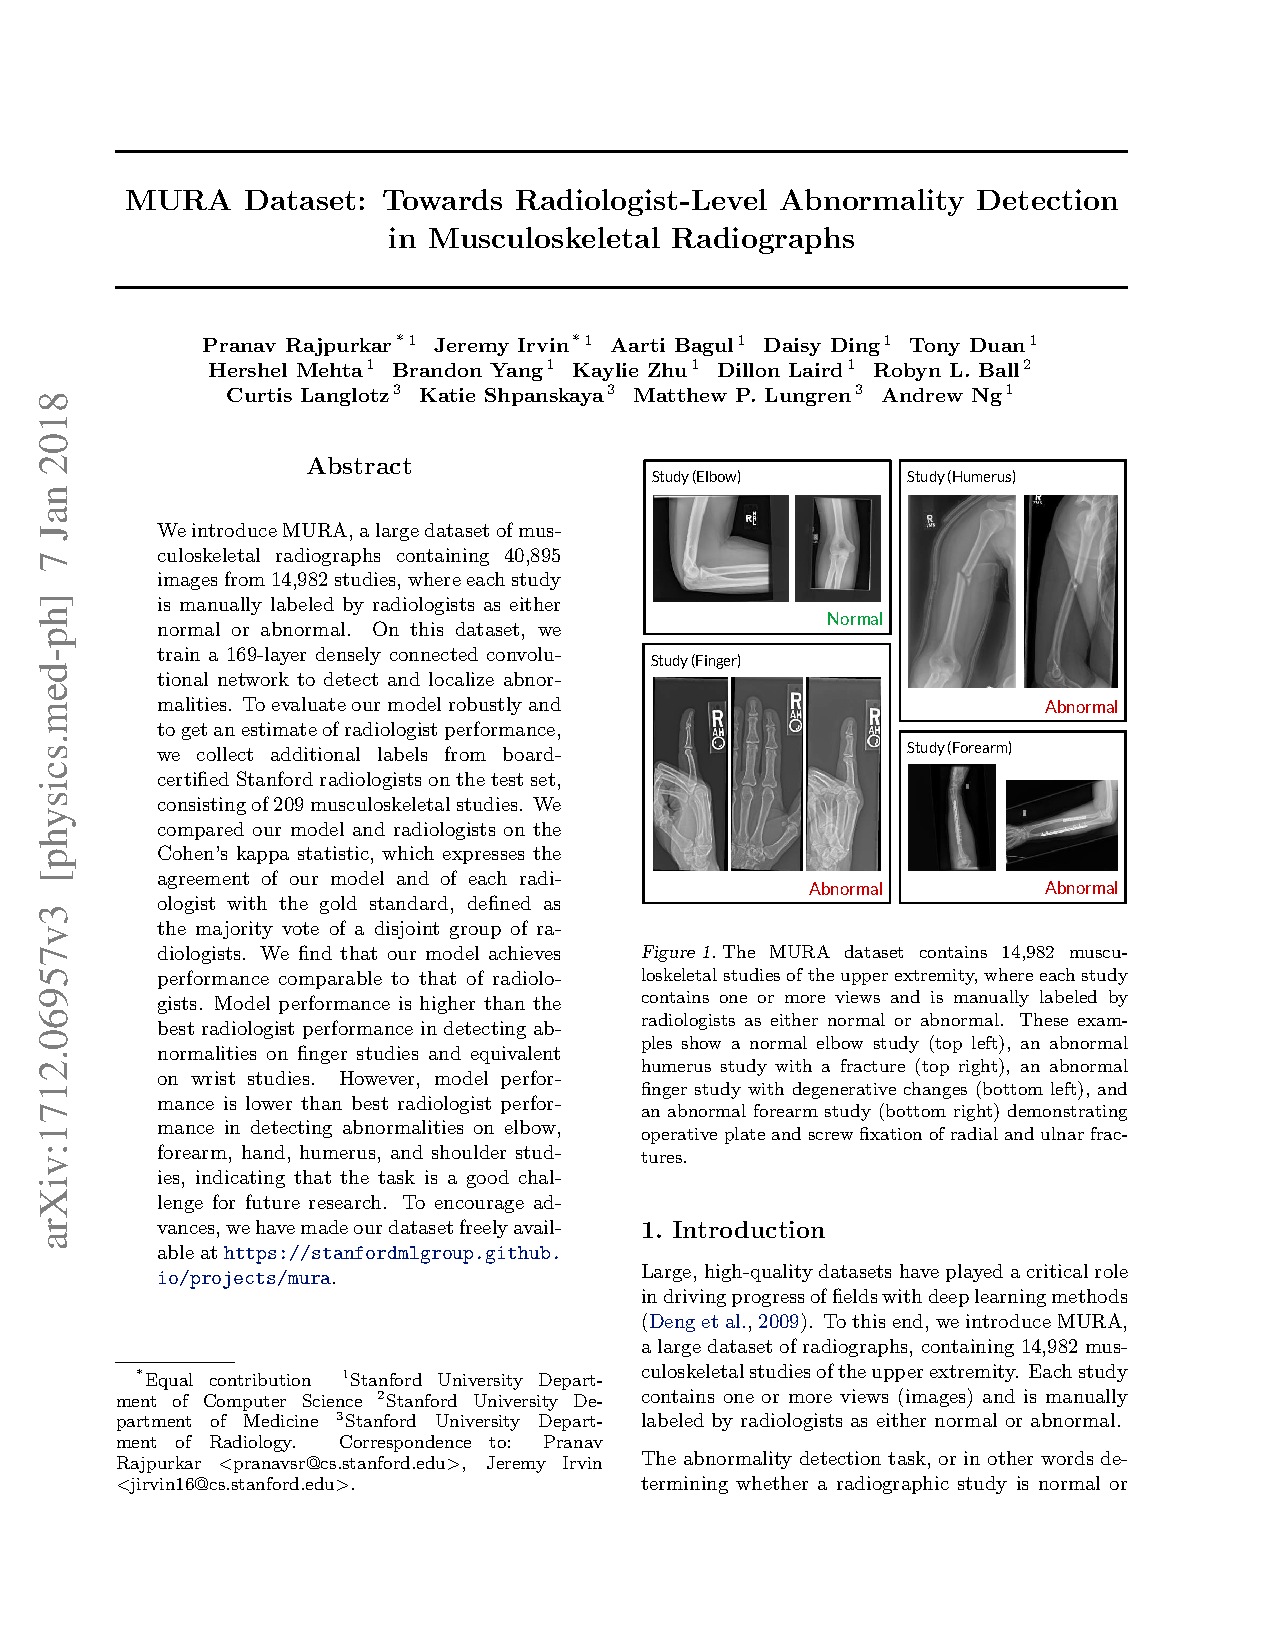
\includegraphics[
                    page=1,
                    width=\textwidth,
                    angle=0,
                    left
                ]{media/mura.pdf}
        \end{minipage}%
        \begin{minipage}{.49\textwidth}%
                \noindent
                \includegraphics[
                    page=2,
                    width=\textwidth,
                    angle=0,
                    right
                ]{media/mura.pdf}
        \end{minipage}%
    }
    \caption{Thumbnail of article by Rajpurkar et al. \autocite{MURA2017}}\label{fig:mura-image}
\end{figure}

MURA is one of the first large radiographic datasets focused exclusively on musculoskeletal imagery, as well as the name of a study conducted alongside said data by the Stanford Center for AI in Medical Imaging \autocite{MURA2017}. The MURA study marks a distinct landmark in the field of AI-assisted fracture classification, because it was the first to apply a deep-learning model on a large (40,561 radiographs), publicly available dataset. As a result, an examination of MURA allows us to contextualise our study in important ways: first, the success of MURA establishes the \emph{possibility} of using deep learning to robustly analyse radiography. Rajpurkar et al.~demonstrates near-radiologist levels of performance, validating the feasibility of our project in general. Secondly, the fact that the MURA model takes multi-view input imagery will help inform our own architectural design for processing both lateral and antero-posterior data. Finally, the limitations of MURA being a pure anomaly-detection system allows us to understand the need for a model which goes beyond binary classification, i.e.~what our project is trying to accomplish. 

To begin, it will be useful to look at MURA's architecture The MURA model is a 169-layer convolutional neural network which takes one or more views as input\footnote{Different views are radiographs of the same subject taken at different standard perspectives.}, and delivers a \emph{probability of anomaly}. The final probability is the arithmetic mean of output probabilities from every view \autocite{MURA2017}. Every type of radiograph may have multiple standard views, and the model architect has a choice of either training a model on a single view, or combining information from views in some ensemble stage. For anomaly detection, MURA chose a fairly conservative approach of assessing a separate probability of anomaly for each view, and then finding their average. This approach will be similar to the one that our project must take: which is to look at both the lateral and anteroposterior view of the tibia.

Another aspect of MURA that is worth examining, is their evaluation process. The model was accessed in two different ways: first, the model's precision versus recall plotted out in a Receiver Operating Characteristic (ROC) plot, and then the Area-Under-Curve of the ROC (AUROC) was quantified.  
\label{AUROC}
The AUROC is a common metric to assess diagnostic ability since it serves to quantify the precision-recall curve of the model. The MURA model had an AUROC of $0.929$. 
Second, a panel of three radiologists were assembled to evaluate a set of radiographs, and their performance was compared against the model. This kind of competitive evaluation allowed the study to compare the model performance against human clinicians, yielding an informative baseline for the AUROC.
With this information, we can contextualise the earlier AUROC value of $0.929$, and see that the model performs slightly worse than humans.

The use of AUROC as an evaluative metric, as well as competitive evaluation with human clinicians, present an advancement in model evaluation compared with the two earlier studies. However, in practice any AI model in radiography will not aim to replace human radiologists entirely, but serve as an additional tool which augments a human clinician's own diagnostic ability. Thus, the MURA study's evaluation is not representative of what real-world deployment would look like. This is why we must turn to Lindsey et al's \emph{Deep neural network improves fracture detection by clinicians}, for a more holistic example of model evaluation.

\section{Lindsey et al: Refinements to Model Evaluation}

\begin{figure}[H]
    \centering
    \fbox{%
        \begin{minipage}{.49\textwidth}%
                \noindent
                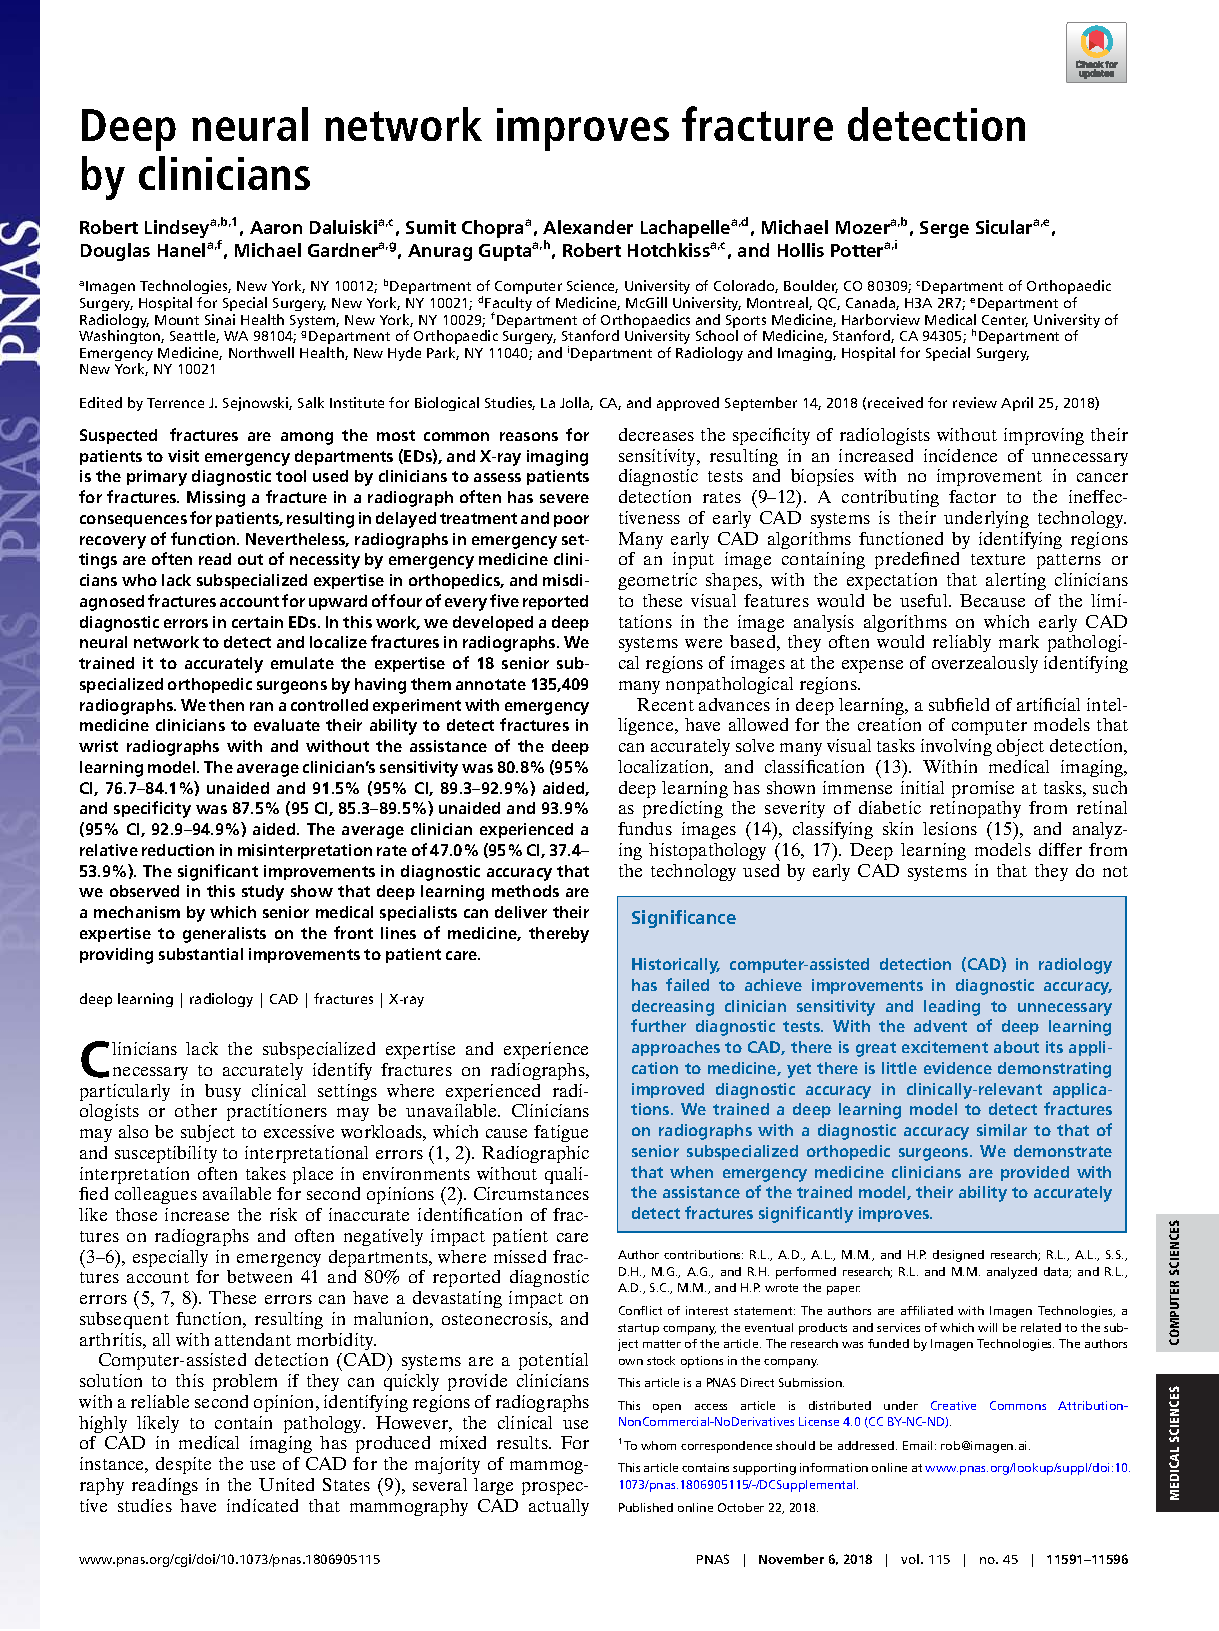
\includegraphics[
                    page=1,
                    width=\textwidth,
                    angle=0,
                    left
                ]{media/lindsey-et-al.pdf}
        \end{minipage}%
        \begin{minipage}{.49\textwidth}%
                \noindent
                \includegraphics[
                    page=2,
                    width=\textwidth,
                    angle=0,
                    right
                ]{media/lindsey-et-al.pdf}
        \end{minipage}%
    }
    \caption{Thumbnail of article by Lindsey et al. \autocite{Lindsey2018}}
    \label{fig:lindsey-image}
\end{figure}

In this study, a deep convolutional neural network is trained on a dataset of 31,490 wrist radiographs \autocite{Lindsey2018}. Like MURA, the study presents an AI-based fracture detection model, outputting both labels as well as a location heatmap. We include this study in the background research, for it's more holistic approach to evaluation, which simulates a real-world use-case. \textcquote{Lindsey2018}{Radiographic interpretation often takes place in environments without qualified colleagues available for second opinions}, the paper acknowledges, before proposing a model which aims to serve a possible \enquote*{second opinion.} After an initial evaluation which demonstrated an AUROC of $0.967$ on certain datasets\footnote{For model testing, the study utilised two distinct categories of radiographs divided into \enquote*{Test Set 1} and \enquote*{Test Set 2} (a slight improvement over MURA), with the former containing a collection of singleton wrist radiographs, and the latter of wrist radiographs with anterio-posterior and lateral views.}, Lindsey et al.~proceeds to conduct a second experiment, where a group of clinicians were shown radiographs from the same test set, and tasked to evaluate the radiograph both with and without the model's assistance:

\pagebreak
\blockcquote{Lindsey2018}{
    For each radiograph shown, the clinicians were asked whether or not
    a fracture was present. After a clinician made a response, the model's
    semantic segmentation prediction [i.e.~heatmap] was shown overlaid on the radiograph;
    the model's clinical determination was shown as text, and the clinician was asked the same question again.
}

\noindent
This experiment simulates the workflow of a clinician when using a fracture-detection model as a part of a CAD workflow. By doing so, we evaluate the effectiveness of the model as an useful tool within a broader clinical practice. The study found that the \textcquote{Lindsey2018}{\ldots\ sensitivity and specificity of the emergency medicine MDs were significantly improved with the assistance of the deep learning model.}

The key advantage of Lindsey et al's paper lies in its evaluative design, which our own project must take inspiration from. It may be impractical to setup a similar trial involving radiologists or clinical professionals,\footnote{Such an addition to this project is, however, within the realm of possibility, in collaboration with the medical faculty at METRC.} but one feature that we do aim to replicate is the output of a heatmap which highlights the location of features that the model detects. For the Lindsey et al.~and the MURA study, these heatmaps highlighted fracture-sights, whereas for our project they will highlight the sites of callus formation and bridging. By having this as a output, we will make the model's behaviour much more interpretable, and allow for integration into real clinical workflows.

\section{Kim \& MacKinnon: Cross-Domain Transfer Learning}

\begin{figure}[H]
    \centering
    \fbox{%
        \begin{minipage}{.49\textwidth}%
                \noindent
                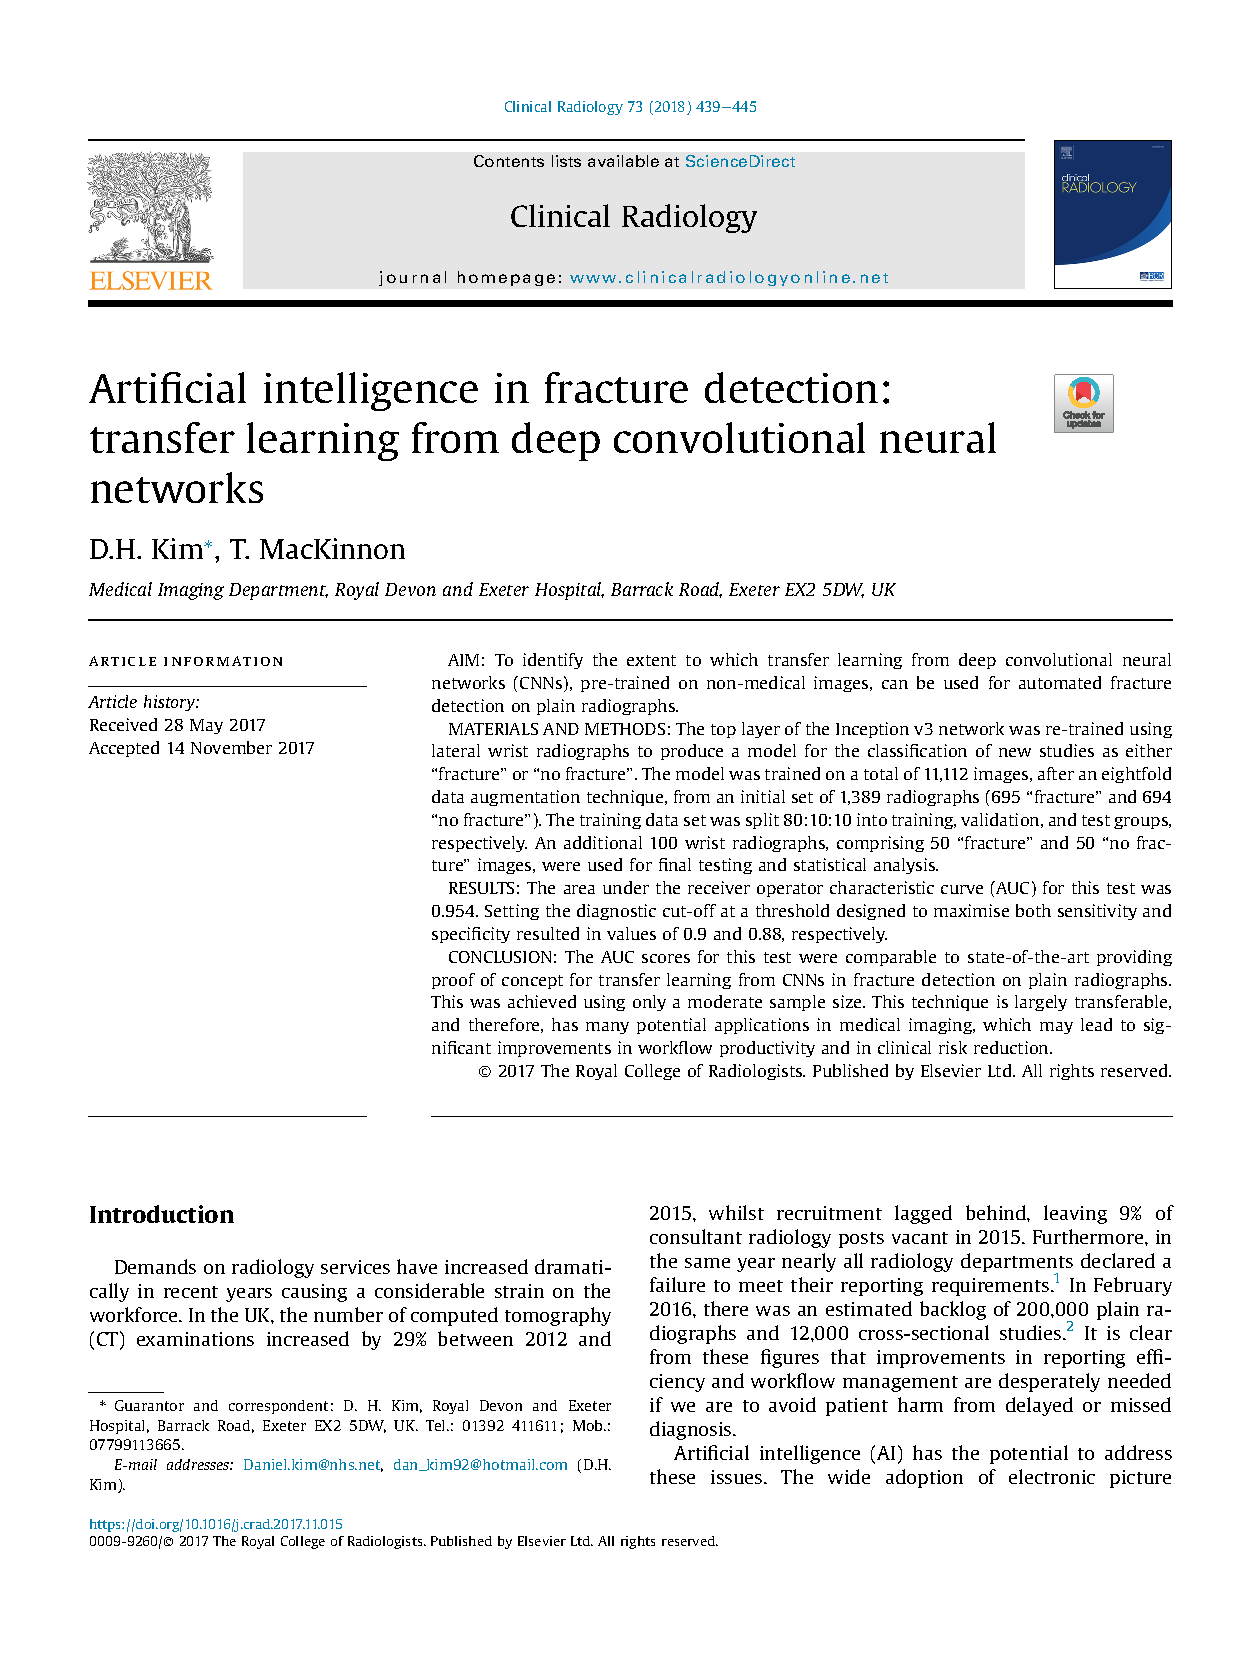
\includegraphics[
                    page=1,
                    width=\textwidth,
                    angle=0,
                    left
                ]{media/kim-and-mackinnon.pdf}
        \end{minipage}%
        \begin{minipage}{.49\textwidth}%
                \noindent
                \includegraphics[
                    page=2,
                    width=\textwidth,
                    angle=0,
                    right
                ]{media/kim-and-mackinnon.pdf}
        \end{minipage}%
    }
    \caption{Thumbnail of article by Kim and MacKinnon. \autocite{Kim2018}}\label{fig:kim2018-image}
\end{figure}  

Studies \autocites{MURA2017}{Lindsey2018} both rely on large, labelled radiographic datasets. While such datasets exist for fracture \emph{detection} and fracture 
\emph{classification}, the classification of fracture healing by their RUST scores is without precedence in literature, and to our knowledge there are no openly available datasets with the aforementioned labels. For our project, we will be using radiographic data internally collected by the \href{https://www.metrc.org/}{Major Extremity Trauma Research Consortium} (METRC), a research unit at the Johns Hopkins Bloomberg School of Public Health. Although this dataset has the RUST-scores we require, the number of radiographs we have access to is limited. Hence our approach is to utilise \emph{transfer learning}, a process where the model is first trained on a larger, general-purpose dataset, before being fine-tuned on the study data. Thus, we turn to Kim and MacKinnon's \emph{Artificial intelligence in fracture detection} for their innovative use of transfer learning.~\autocite{Kim2018}

In Kim and MacKinnon's study, a dataset of 1,389 radiographs was available for a binary classification task (i.e.~labels were \enquote{fracture} or \enquote{no fracture}). Instead of training a model \emph{ab initio}, a CNN trained on a general purpose, non-radiographic dataset was re-applied on the radiography data. The authors used the Inception v3 network, an object-detection and image classification network  \autocite{Szegedy2016} with the topmost layer fine-tuned on the radiographic data. \autocite{Kim2018}. By using a pre-existing model and data augmentation\footnote{The authors of \autocite{Kim2018} ultimately generated 11,112 augmented samples from their initial set of 1,389 radiographs.}, Kim and MacKinnon were able to achieve an  AUROC of $0.954$, a value that is within the same standard deviation of \autocites{MURA2017}{Lindsey2018}, studies which both had much larger datasets for their models.

Our inclusion of Kim and MacKinnon's study serves as an important validation for the aims of our project. The METRC dataset will consist of around two to three thousand radiographs sourced from a handful of METRC studies. If Kim and MacKinnon's model is already able to achieve a robust performance with only 1,389 samples, than it is quite possible for our own project to achieve it's aims. The theoretical reasoning behind why transfer learning can achieve high levels of model performance is because the first layers of a CNN are primarily responsible for high-level feature extraction, e.g.~edge detection, pattern recognition, with only the latter layers responsible for task-specific classification \autocite{Kim2018}. This does, however open up a further avenue of inquiry. Would model performance improve further, if the base model that the transfer learning is conducted from, was itself originally trained on a domain-specific dataset, like the MURA data from \autocite{MURA2017}? Our project will explore this possibility, through it's own application of transfer learning to the prediction of radiographic union with RUST scores.

% I should look at three different papers in depth.

% This one also looks at AT/L views
% https://pubmed.ncbi.nlm.nih.gov/30348771/

% MURA: Large dataset
% https://arxiv.org/pdf/1712.06957.pdf

% Transfer Learning
%  https://www.clinicalradiologyonline.net/article/S0009-9260(17)30535-4/fulltext
